%%%%%%%%%%%%%%%%%%%%%%%%%%%%%%%%%%%%%%%%%
% a0poster Landscape Poster
% LaTeX Template
% Version 1.0 (22/06/13)
%
% The a0poster class was created by:
% Gerlinde Kettl and Matthias Weiser (tex@kettl.de)
% 
% This template has been downloaded from:
% http://www.LaTeXTemplates.com
%
% License:
% CC BY-NC-SA 3.0 (http://creativecommons.org/licenses/by-nc-sa/3.0/)
%
%%%%%%%%%%%%%%%%%%%%%%%%%%%%%%%%%%%%%%%%%

%----------------------------------------------------------------------------------------
%	PACKAGES AND OTHER DOCUMENT CONFIGURATIONS
%----------------------------------------------------------------------------------------

\documentclass[a0,landscape]{a0poster}

\usepackage{multicol} % This is so we can have multiple columns of text side-by-side
\columnsep=100pt % This is the amount of white space between the columns in the poster
\columnseprule=3pt % This is the thickness of the black line between the columns in the poster

\usepackage[svgnames]{xcolor} % Specify colors by their 'svgnames', for a full list of all colors available see here: http://www.latextemplates.com/svgnames-colors

\usepackage{times} % Use the times font
%\usepackage{palatino} % Uncomment to use the Palatino font

\usepackage{graphicx} % Required for including images
\graphicspath{{figures/}} % Location of the graphics files
\usepackage{booktabs} % Top and bottom rules for table
\usepackage[font=small,labelfont=bf]{caption} % Required for specifying captions to tables and figures
\usepackage{amsfonts, amsmath, amsthm, amssymb} % For math fonts, symbols and environments
\usepackage{wrapfig} % Allows wrapping text around tables and figures

\begin{document}

%----------------------------------------------------------------------------------------
%	POSTER HEADER 
%----------------------------------------------------------------------------------------

% The header is divided into three boxes:
% The first is 55% wide and houses the title, subtitle, names and university/organization
% The second is 25% wide and houses contact information
% The third is 19% wide and houses a logo for your university/organization or a photo of you
% The widths of these boxes can be easily edited to accommodate your content as you see fit

\begin{minipage}[b]{0.55\linewidth}
\veryHuge \color{NavyBlue} \textbf{Sign Language Recognition} \color{Black}\\ % Title
\Huge\textit{}\\[1cm] % Subtitle
\huge \textbf{Mukesh Makwana \& Rathna G. N}\\ % Author(s)
\huge Indian Institute of Science\\
Electrical Engineering\\ % University/organization
\end{minipage}
%
\begin{minipage}[b]{0.25\linewidth}
\color{DarkSlateGray}\Large \textbf{Contact Information:}\\
DSP Lab\\
Electrical Engineering\\ % Address
Indian Institute of Science\\
Bangalore, Karnataka, India\\\\
Phone: +91 8880 994668\\ % Phone number
Email: \texttt{mux032@gmail.com}\\ % Email address
\end{minipage}
%
\begin{minipage}[b]{0.19\linewidth}

\includegraphics[width=13cm]{logo.png} % Logo or a photo of you, adjust its dimensions here
\end{minipage}

\vspace{1cm} % A bit of extra whitespace between the header and poster content

%----------------------------------------------------------------------------------------

\begin{multicols}{4} % This is how many columns your poster will be broken into, a poster with many figures may benefit from less columns whereas a text-heavy poster benefits from more

%----------------------------------------------------------------------------------------
%	ABSTRACT
%----------------------------------------------------------------------------------------

\color{Navy} % Navy color for the abstract

% \begin{abstract}

% \textbf{S}ign language recognition is required to efficiently fill the communication gap between hearing-impaired minority and hearing majority. We consider the problem of designing a Sign Language recognition system that takes the image of hand-signed alphabet as an input and returns the recognized character.

% \end{abstract}

%----------------------------------------------------------------------------------------
%	INTRODUCTION
%----------------------------------------------------------------------------------------

\color{SaddleBrown} % SaddleBrown color for the introduction

\section*{Introduction}

\textbf{C}ommunication between hearing-impaired minority and non-impaired majority is difficult as most of the time latter community is not aware of sign language.\\
\indent \textbf{S}ign language consists of two major components namely Finger-spelling and Word level sign vocabulary. Finger-spelling is used to spell words letter by letter, whereas Word level sign vocabulary comprises of signed words and is used for the majority of communication. \\
\indent \textbf{F}inger-spelling recognition can be broadly divided into two parts, extraction of feature vectors and classification of gestures using feature vectors. The two dataset used both contains depth images of gestures. The use of depth images eases the task of preprocessing and helps obtain results in real-time.
%----------------------------------------------------------------------------------------
%	OBJECTIVES
%----------------------------------------------------------------------------------------

\color{DarkSlateGray} % DarkSlateGray color for the rest of the content

% \section*{Main Objectives}

% \begin{enumerate}
% \item Lorem ipsum dolor sit amet, consectetur.
% \item Nullam at mi nisl. Vestibulum est purus, ultricies cursus volutpat sit amet, vestibulum eu.
% \item Praesent tortor libero, vulputate quis elementum a, iaculis.
% \item Phasellus a quam mauris, non varius mauris. Fusce tristique, enim tempor varius porta, elit purus commodo velit, pretium mattis ligula nisl nec ante.
% \item Ut adipiscing accumsan sapien, sit amet pretium.
% \item Estibulum est purus, ultricies cursus volutpat
% \item Nullam at mi nisl. Vestibulum est purus, ultricies cursus volutpat sit amet, vestibulum eu.
% \item Praesent tortor libero, vulputate quis elementum a, iaculis.
% \end{enumerate}

%----------------------------------------------------------------------------------------
%	MATERIALS AND METHODS
%----------------------------------------------------------------------------------------

\section*{Datasets}

First dataset used is ASL dataset collected by Byeongkeun \textit{et al.} contains 31,000 images from five different subjects for 31 different gestures from each. 

%------------------------------------------------

\begin{center}\vspace{1cm}
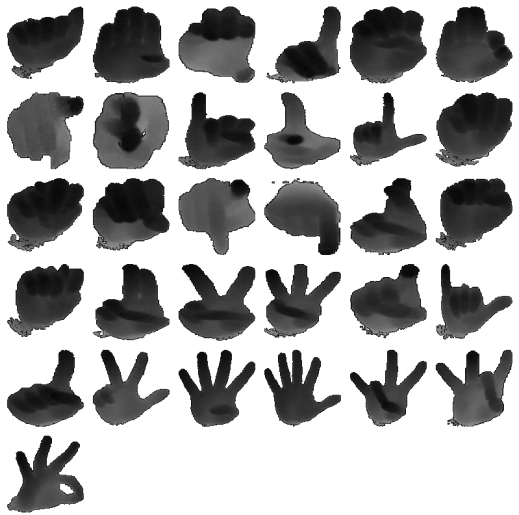
\includegraphics[width=0.7\linewidth]{processed}
\captionof{figure}{\color{Green} ASL Dataset (Depth Images)}
\end{center}\vspace{1cm}

Second dataset is ISL dataset which has been collected by us, it contains 630 images from six different subjects for five gestures from each.
\begin{center}\vspace{1cm}
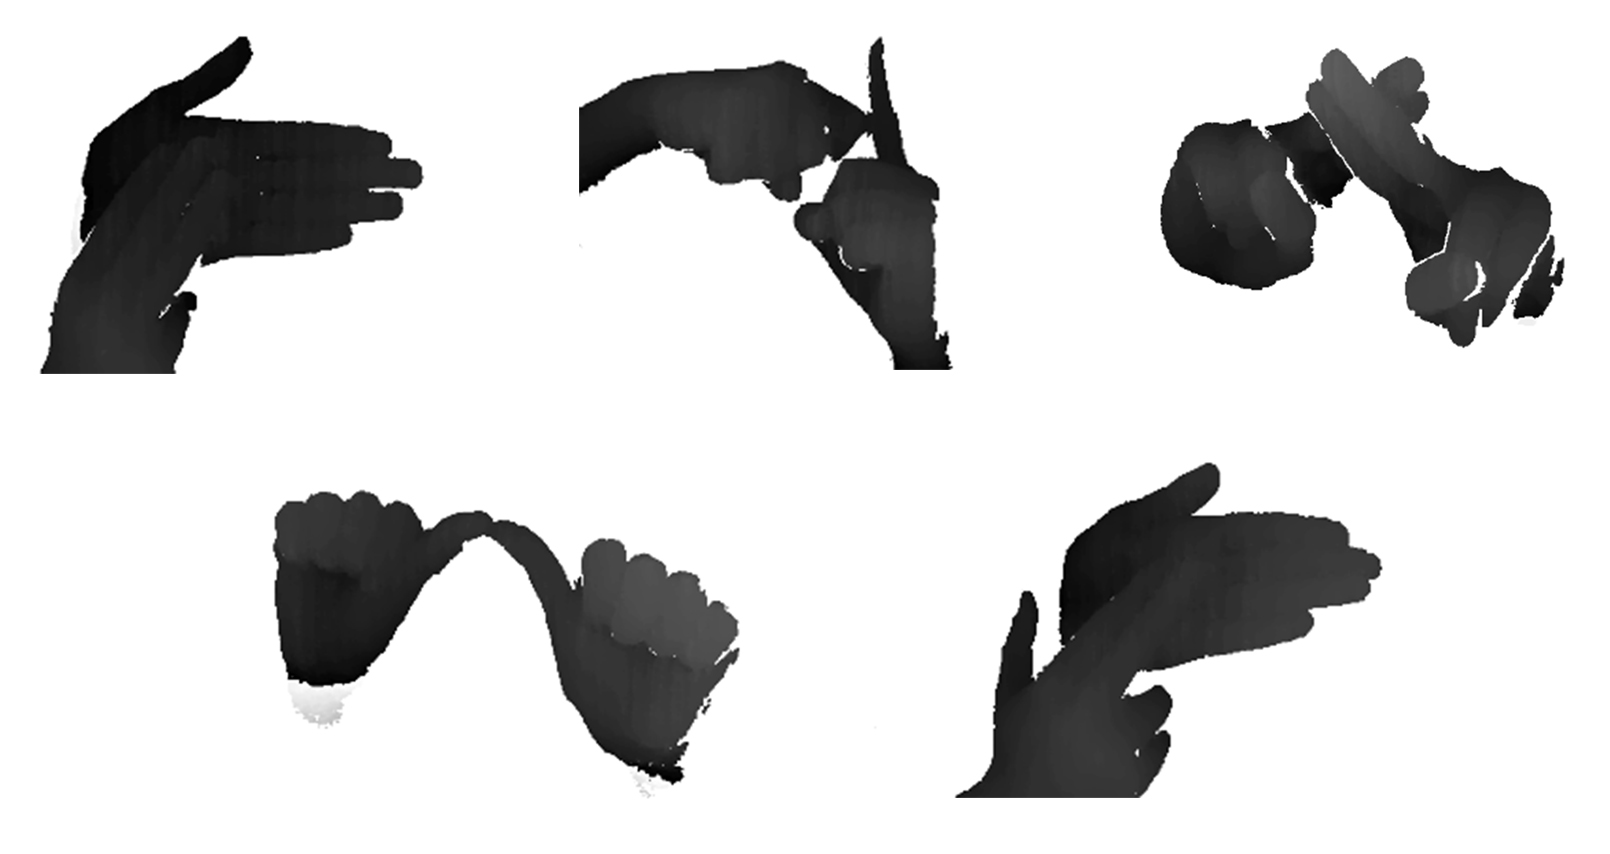
\includegraphics[width=0.70\linewidth]{isl1}
\captionof{figure}{\color{Green} ISL Dataset (Depth Images)}
\end{center}\vspace{1cm}

\section*{Methods}

Few methods which are used for ASL dataset and ISL dataset are:\\

\begin{itemize}
\item \textbf{Random Forest:} Its an estimator that operates on a number of decision tree classifiers on various subsamples (using bootstrap aggregating) of the dataset.
\begin{center}\vspace{1cm}
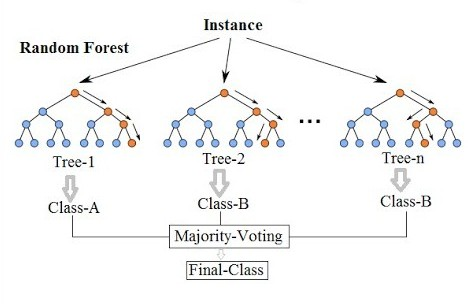
\includegraphics[width=0.99\linewidth]{rf}
\captionof{figure}{\color{Green} Random Forest}
\end{center}\vspace{1cm}

\item \textbf{SVM:} SVM finds an optimal hyperplane between different classes. Principal Component Analysis (PCA) is applied before SVM model for dimensionality reduction.

\begin{center}\vspace{1cm}
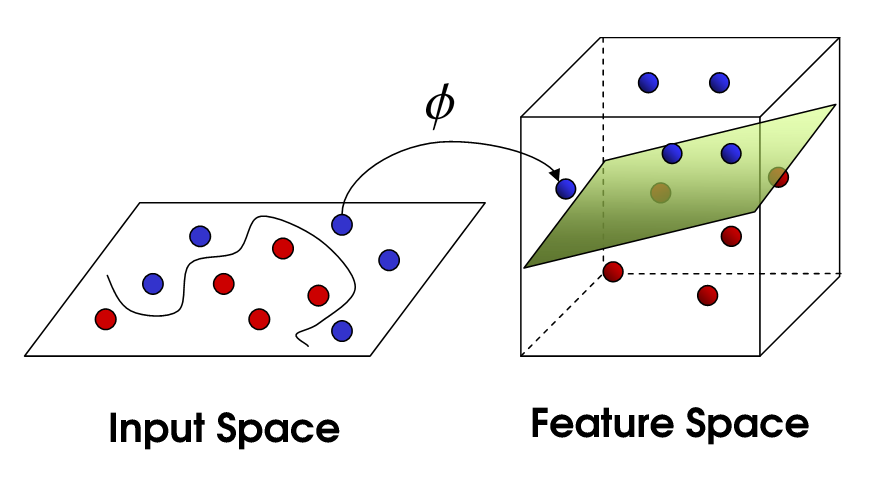
\includegraphics[width=0.99\linewidth]{svm}
\captionof{figure}{\color{Green} SVM for two classes}
\end{center}\vspace{1cm}

\item \textbf{CNN:} Convolutional Neural Network is a deep neural network which uses the property of convolution. One important advantage of CNN over ordinary NN is the reduction in the number of parameters to be learnt. A CNN primarily consists of convolution layer, ReLU layer and Pooling layer. ReLU is an activation function layer. Pooling performs the down sampling operation and reduces the volume of output of ReLU.
\end{itemize}
\vspace{1cm}

\begin{center}\vspace{1cm}
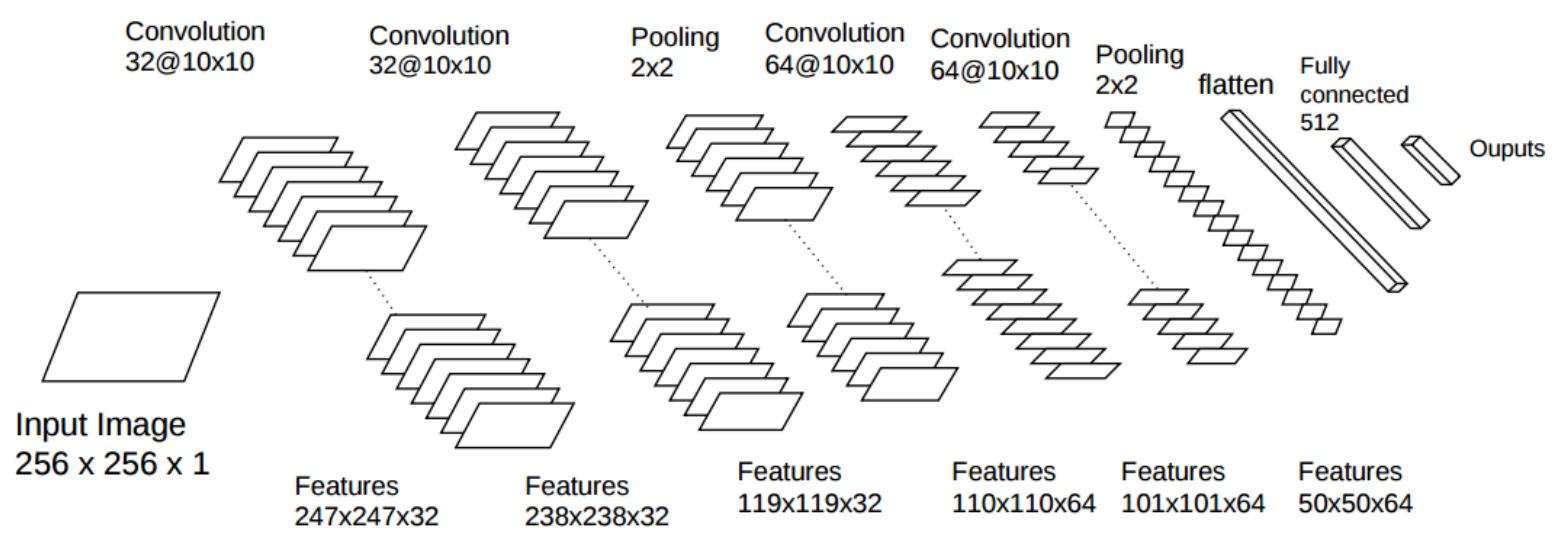
\includegraphics[width=0.99\linewidth]{cnn}
\captionof{figure}{\color{Green} Convolutional Neural Network}
\end{center}\vspace{1cm}
%----------------------------------------------------------------------------------------
%	RESULTS 
%----------------------------------------------------------------------------------------
\section*{Results}

For ASL Dataset, we trained our models on four subjects and tested on fifth subject . And after taking all combination of subjects we get the average accuracy value. Accuracies are noted below in table,


\begin{center}\vspace{1cm}
\begin{tabular}{@{}lccc@{}}
\toprule
Method & \multicolumn{1}{l}{\textbf{\# of Sub.}} & \multicolumn{1}{l}{\textbf{\# of class}} & \multicolumn{1}{l}{\textbf{Accur.(\%)}} \\ \midrule
\multicolumn{1}{|l|}{\textbf{SVM (4/1)}} & \multicolumn{1}{c|}{5} & \multicolumn{1}{c|}{31} & \multicolumn{1}{c|}{48.01} \\ \midrule
\textbf{RF (4/1)} & 5 & 31 & 70 \\ \midrule
\multicolumn{1}{|l|}{\textbf{CNN (4/1)}} & \multicolumn{1}{c|}{5} & \multicolumn{1}{c|}{31} & \multicolumn{1}{c|}{70$\pm$1} \\ \bottomrule
\end{tabular}
\end{center}
\vspace{3cm}*
Diagonal of Confusion matrix plot shows the number of gestures which are perfectly classified (darkest in diagonal) and those which are confused with other gestures (faint in diagonal).

\begin{center}\vspace{1cm}
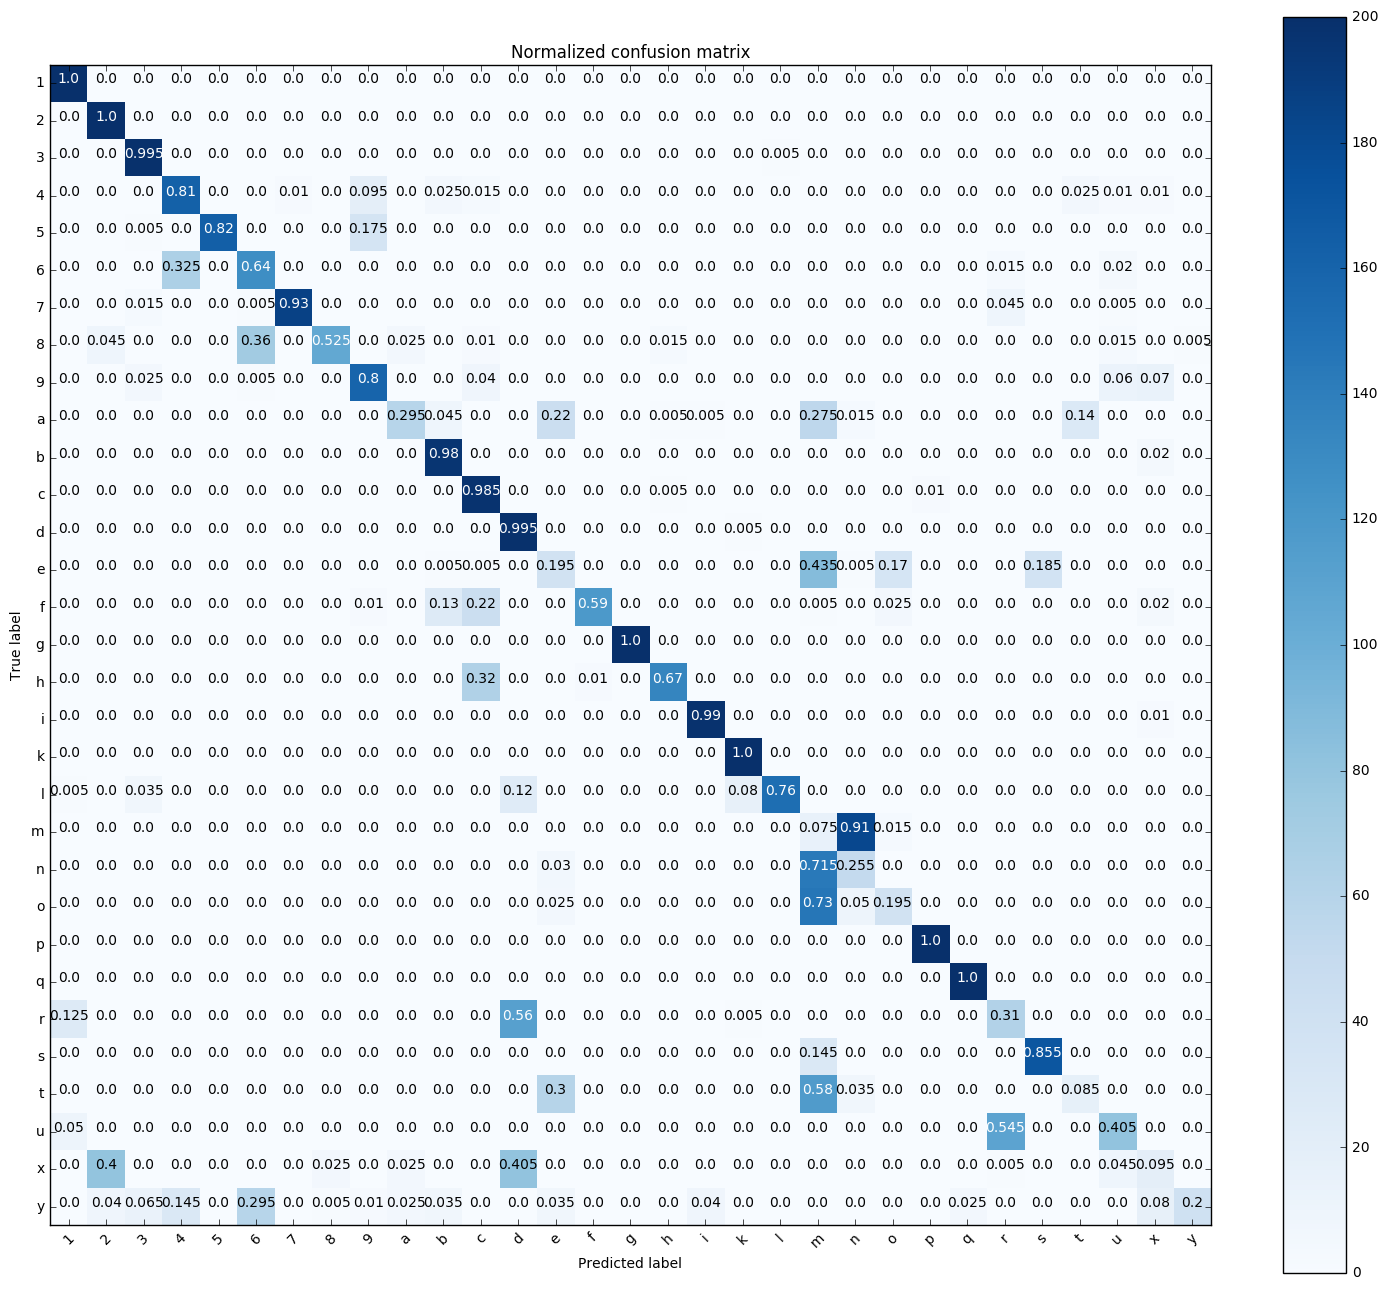
\includegraphics[width=0.90\linewidth]{cm_normalized}
\captionof{figure}{\color{Green} Confusion Matrix}
\end{center}\vspace{1cm}

\begin{center}\vspace{1cm}
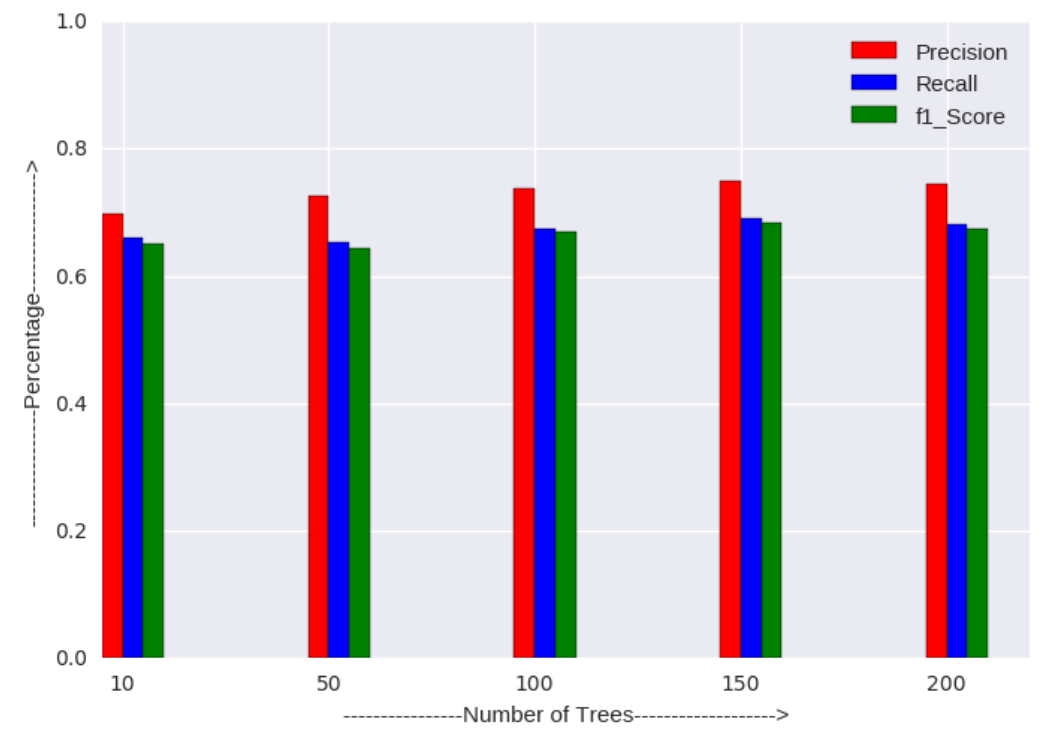
\includegraphics[width=0.90\linewidth]{f1}
\captionof{figure}{\color{Green} Random Forest with different numbers of trees}
\end{center}\vspace{1cm}

For ISL dataset, we trained our models on five subjects and tested on 6th subject. And after taking all combination of subjects we get the average accuracy value. Accuracies are noted below in table,

\begin{center}\vspace{1cm}

\label{my-label}
\begin{tabular}{@{}lccc@{}}
\toprule
Method & \multicolumn{1}{l}{\textbf{\# of Sub.}} & \multicolumn{1}{l}{\textbf{\# of class}} & \multicolumn{1}{l}{\textbf{Accur.(\%)}} \\ \midrule
\multicolumn{1}{|l|}{SVM (5/1)} & \multicolumn{1}{c|}{6} & \multicolumn{1}{c|}{5} & \multicolumn{1}{c|}{98} \\ \midrule
RF (5/1) & 6 & 5 & 68.7 \\ \midrule
\multicolumn{1}{|l|}{CNN (5/1)} & \multicolumn{1}{c|}{6} & \multicolumn{1}{c|}{5} & \multicolumn{1}{c|}{83.7} \\ \bottomrule
\end{tabular}
\end{center}

%----------------------------------------------------------------------------------------
%	CONCLUSIONS
%----------------------------------------------------------------------------------------

\color{SaddleBrown} % SaddleBrown color for the conclusions to make them stand out

\section*{Conclusions}

\begin{itemize}
\item SVM and Random forest are better with training time and accuracy, but there is a very little to no room for further improvement and it cannot be trained dynamically.  
\item Whereas CNN takes much time to train and requires a large dataset for efficiency. But can be trained on new dataset on-the-go. Further tweaking properly, might result in better accuracy than achieved so far. 
\end{itemize}

\color{DarkSlateGray} % Set the color back to DarkSlateGray for the rest of the content

%----------------------------------------------------------------------------------------
%	FORTHCOMING RESEARCH
%----------------------------------------------------------------------------------------

\section*{Forthcoming Research}
\begin{itemize}
\item Significant improvement must be made in resolving the ambiguity in detection of visually similar alphabets. for example {a, e, m, n, o, s, t}.
\item The problem statement can be extended to word detection using fingerspelling in real-time.
\end{itemize}

 %----------------------------------------------------------------------------------------
%	REFERENCES
%----------------------------------------------------------------------------------------
\section*{References}

% \nocite{*} % Print all references regardless of whether they were cited in the poster or not
% \bibliographystyle{plain} % Plain referencing style
% \bibliography{sample} % Use the example bibliography file sample.bib
\begin{enumerate}
\item Byeongkeun Kang, Subarna Tripathi, and Truong Q. Nguyen. Real-time Sign Language Fingerspelling Recognition using Convolutional Neural Networks from Depth map. Department of Electrical and Computer Engineering, San Diego, 2015.
\end{enumerate}
%----------------------------------------------------------------------------------------
%	ACKNOWLEDGEMENTS
%----------------------------------------------------------------------------------------

%\section*{Acknowledgements}

%Etiam fermentum, arcu ut gravida fringilla, dolor arcu laoreet justo, ut imperdiet urna arcu a arcu. Donec nec ante a dui tempus consectetur. Cras nisi turpis, dapibus sit amet mattis sed, laoreet.

%----------------------------------------------------------------------------------------

\end{multicols}
\end{document}